
\documentclass[10pt]{article}

% ============================================================
% AMOS Paper Settings
% ============================================================
\usepackage[margin=1in]{geometry}
\usepackage{times}
\usepackage{microtype}
\usepackage{amsmath}
\usepackage{amssymb}
\usepackage{booktabs}
\usepackage{array}
\usepackage{enumitem}
\usepackage{longtable}
\usepackage{graphicx}
\usepackage{float}
\usepackage{xcolor}
\usepackage{url}
\usepackage{xspace}
\usepackage{tikz}
\usetikzlibrary{arrows.meta,fit,positioning}
\usepackage[hidelinks]{hyperref}
\hypersetup{
  pdftitle={AMOS: A Memory Operating Layer for Autonomous Data Analysis},
  pdfauthor={Elton Chang}
}

\setlist[itemize]{leftmargin=1.2em, itemsep=0.2em, topsep=0.2em}
\setlist[enumerate]{leftmargin=1.4em, itemsep=0.25em, topsep=0.25em}
\newcolumntype{L}[1]{>{\raggedright\arraybackslash}p{#1}}
\newcolumntype{C}[1]{>{\centering\arraybackslash}p{#1}}
\renewcommand{\arraystretch}{1.08}
\newcommand{\amos}{\textsc{AMOS}\xspace}
\newcommand{\mem}{\mathcal{M}}
\newcommand{\task}{\mathcal{T}}
\newcommand{\claim}{\mathcal{C}}
\newcommand{\prov}{\mathcal{G}}
\newcommand{\code}[1]{\texttt{#1}}
\newcommand{\yes}{\textbf{Yes}}
\newcommand{\partly}{Partly}
\newcommand{\none}{--}
\newcommand{\na}{n/a}
\newcommand{\pass}{\textbf{Pass}}
\newcommand{\fail}{Fail}

\title{AMOS: A Memory Operating Layer for Autonomous Data Analysis}
\author{Elton Chang}
\date{}

\begin{document}
\maketitle

\begin{abstract}
Continuous large-scale data analysis agents operate across warehouses, streams, catalogs, semantic layers, documents, notebooks, and prior investigations. Their reliability depends not only on model reasoning, but on continuously managing the state that makes each computation valid: schema and metric versions, snapshots or stream offsets, freshness, permissions, feedback, execution records, and provenance. Prompt context, RAG, and text-to-SQL address parts of this problem but do not provide a durable operating abstraction for analytical state.

\amos is a memory operating layer between data analysis agents and the systems they use. It separates bounded model-visible context from persistent, typed, versioned memory; filters permissions before context construction; reconciles temporal and authority conflicts; verifies computations against current schema and semantic state; and attaches claim-level provenance and replay metadata after execution. Raw data remains in existing data platforms while \amos manages governed metadata, references, and analytical history through a stable runtime protocol.

We formalize the memory operating layer, implement a reference system, and evaluate its correctness, auditability, and scaling behavior. \amos matches all outcomes in a 12-task invariant benchmark, compared with 6 of 12 for the strongest local baseline. Across payment failure, subscription churn, and warehouse quality, it satisfies all twelve seeded capability-contract variants per domain in three deterministic repetitions. Component ablations isolate the contribution of verification, permission filtering, and provenance. Indexed studies cover 1{,}000{,}001 memory objects and 1{,}000{,}000 provenance edges, while a governed BM25, MiniLM/HNSW, and hybrid comparison quantifies retrieval quality and latency through 100k distractors with zero restricted-item or superseded-item leaks. The results establish a concrete systems foundation for continuous large-scale data analysis agents whose context, computation, claims, and corrections remain governable over time.
\end{abstract}

\section{Introduction}

Language-model agents increasingly perform continuous data analysis: they translate questions into SQL, execute notebooks, inspect documents, monitor dashboards, and generate reports. At organizational scale, each task crosses changing data and metadata systems, and fluent output can hide state errors such as stale metrics, wrong schemas, incomplete late data, unauthorized evidence, or superseded analyses. The central systems problem is how an agent maintains the valid analytical state for every computation as workloads, users, and source systems evolve.

Continuous large-scale analysis is stateful. A request such as ``why did anomaly rate increase in the last six hours?'' may require an approved metric, stream offsets and watermarks, an active schema, ingestion delays, prior incidents, quality checks, and the query or chart supporting each claim. Existing data systems provide pieces of this state \cite{millwheel,dataflow,flink,deltalake,openlineage,provdm}; an analytical agent still needs an operating layer that selects valid context, resolves conflicts, preserves corrections, and ties outputs back to execution evidence across tasks.

Existing LLM techniques are building blocks, not a full memory abstraction. RAG exposes external text \cite{rag}; long-context models remain position-sensitive \cite{lostinthemiddle}; tool-using agents interleave reasoning and actions \cite{react,toolformer}; text-to-SQL benchmarks measure schema-grounded queries \cite{spider,bird,spider2}. None guarantees temporally valid, permission-filtered, conflict-aware context linked to reproducible execution traces.

\amos is that memory operating layer. It sits between analysis agents and warehouses, stream processors, semantic layers, catalogs, documents, execution tools, and lineage systems. These systems provide data, definitions, or traces; \amos gives agents one runtime contract for deciding which versioned and permissioned state enters a bounded working set, verifying computation against that state, recording claim support, and carrying reviewed corrections into later tasks.

\paragraph{System boundary.} \amos manages analytical state and references rather than copying unrestricted raw data into model memory. It targets controllable validity, governance, and auditability: analysts retain responsibility for causal and high-impact decisions, while every important claim remains inspectable through its data state, computation, definitions, memory versions, and verification record.

\paragraph{Contributions.} The paper contributes:
\begin{enumerate}
    \item a systems abstraction for a memory operating layer that connects continuous analysis agents to changing data, semantic, governance, and execution state;
    \item a typed hierarchy and runtime protocol for bounded retrieval, supersession, reconciliation, verification, citation, feedback, and replay;
    \item claim-level provenance linking outputs to data state, code, definitions, memory versions, permissions, and verification status;
    \item a reference implementation and reproducible evaluation spanning invariant coverage, three analytical domains, component ablations, retrieval engines, concurrency, and million-object local scale.
\end{enumerate}

\paragraph{Research questions.} The evaluation is organized around four questions:
\begin{enumerate}
    \item[RQ1.] \textbf{Operating-layer correctness:} does the runtime accept valid analytical computations and reject schema, metric, permission, freshness, and safety violations?
    \item[RQ2.] \textbf{Persistent contract enforcement:} which guarantees require a memory operating layer rather than prompt-only, retrieval-only, semantic, or lineage policies?
    \item[RQ3.] \textbf{Auditability cost:} what latency, storage, and replay overhead is added by claim-level provenance and governed state management?
    \item[RQ4.] \textbf{Large-scale behavior:} how do indexed memory, provenance, retrieval quality, concurrency, and updates behave as state grows from thousands to millions of objects?
\end{enumerate}

\section{Background and Related Work}

\subsection{Memory, Context, and Operating Layers for LLM Agents}
LLMs operate under finite context windows. Long-context models help, but they still require context selection, ordering, updating, and validation; models may underuse information placed in the middle of long prompts \cite{lostinthemiddle}. MemGPT treats the prompt as constrained main memory and external stores as archival memory \cite{memgpt}. Generative Agents stores observations and reflections for later planning, while Reflexion persists verbal feedback across trials \cite{generativeagents,reflexion}. Surveys organize agent memory by sources, representations, operations, and evaluation strategies \cite{memorysurvey}. \amos extends this line from memory as stored content to memory as an operating layer: a governed interface over schemas, metrics, snapshots, stream offsets, code, feedback, permissions, and provenance that mediates every analytical task.

\subsection{Retrieval, Tool Use, and Text-to-SQL}
RAG retrieves non-parametric evidence \cite{rag}; ReAct and Toolformer show how agents interleave reasoning with tool calls \cite{react,toolformer}; Spider, BIRD, Spider 2.0, and EntSQL evaluate schema grounding, database interaction, enterprise metadata, dialects, codebase context, and business semantics \cite{spider,bird,spider2,entsql}. These directions motivate \amos but leave a gap: query generation alone is insufficient when correctness depends on versioned memory, feedback retention, temporal validity, permissions, and provenance.

\subsection{Streaming, Snapshots, and Reproducible Data States}
Stream-processing systems formalize event time, watermarks, windows, state, and replay \cite{millwheel,dataflow,flink}; lakehouse systems provide transactions and time-travel snapshots \cite{deltalake}. \amos does not reimplement these mechanisms. It records references to the event-time window, watermark, snapshot version, query, and late-data policy used by an analytical claim.

\subsection{Provenance, Lineage, Data Quality, and Security}
PROV and OpenLineage define provenance and lineage vocabularies for entities, jobs, datasets, and runs \cite{provdm,openlineage}. noWorkflow captures definition, deployment, and execution provenance from scripts, while YesWorkflow exposes prospective dataflow from lightweight annotations \cite{noworkflow,yesworkflow}. Data-quality systems show the value of explicit validation constraints and drift checks \cite{deequ,tfdv}. LLM-integrated applications add prompt-injection risk when external content is treated as instructions \cite{owasp,greshake2023indirect,yi2023bipia}. Recent runtime-governance work formalizes policies over partial agent execution paths rather than relying only on prompts or static access checks \cite{runtimegovernance}. \amos specializes this runtime-policy perspective to analytical state and claim support.

\subsection{Positioning Against Existing System Classes}
Table~\ref{tab:comparison} summarizes the boundary between \amos and adjacent systems. In deployment, \amos should rely on them; its role is the runtime policy for selecting, reconciling, verifying, citing, and updating an analytical agent's working state.

The contribution is a compositional systems abstraction rather than a new retrieval algorithm or provenance vocabulary in isolation. The memory operating layer ties effective-time and authority-aware context selection to pre-execution verification, post-execution claim support, durable feedback, and replay through one executable contract.

\begin{table}[t]
\centering
\scriptsize
\setlength{\tabcolsep}{2.8pt}
\begin{tabular}{L{0.20\linewidth}C{0.13\linewidth}C{0.14\linewidth}C{0.14\linewidth}C{0.13\linewidth}C{0.13\linewidth}}
\toprule
\textbf{Runtime capability} & \textbf{RAG} & \textbf{Semantic layer} & \textbf{Catalog/ lineage} & \textbf{Long context} & \textbf{\amos} \\
\midrule
Task evidence retrieval & \yes & \partly & \partly & \yes & \yes \\
Metric version by interval & \partly & \yes & \partly & \none & \yes \\
SQL/schema/policy check & \none & \partly & \partly & \none & \yes \\
Pre-context permission filter & Optional & \partly & \partly & \none & \yes \\
Authority/time reconciliation & \none & \partly & \partly & \none & \yes \\
Claim-level support links & \none & \none & Job-level & \none & \yes \\
Durable reviewer feedback & Optional & \none & \none & \none & \yes \\
Replay with memory/verifier state & \none & \none & Job-level & \none & \yes \\
\bottomrule
\end{tabular}
\caption{Conceptual comparison with adjacent system classes. \none{} denotes no typical standalone support; ``Partly'' denotes support that usually requires additional integration or policy. \amos is intended to compose with these systems rather than replace them.}
\label{tab:comparison}
\end{table}

\section{Continuous Analysis as an Operating-Layer Problem}

\subsection{Continuous Large-Scale Analytical Task}
A simplified text-to-SQL task maps a natural-language request $q$ and schema context $C$ to an executable query $E$:
\begin{equation}
    q + C \rightarrow E.
\end{equation}
For continuous large-scale analytics this abstraction is too small. At time $t$, a task depends on streams, snapshots, schemas, semantic definitions, documents, prior analyses, feedback, and permissions distributed across multiple systems:
\begin{equation}
    \task_t = (q_t, S_{1:n}, H, C_t, D_t, A_{<t}, F_{<t}, P_t),
\end{equation}
where $S_{1:n}$ are streams, $H$ is snapshots, $C_t$ is schema/catalog state, $D_t$ is governed document context, $A_{<t}$ prior analyses, $F_{<t}$ feedback, and $P_t$ the active access policy.

The agent must produce an artifact $Y_t$ and a reproducible support record:
\begin{equation}
    \task_t \rightarrow (Y_t, E_t, \prov_t, R_t),
\end{equation}
where $E_t$ is executable computation, $\prov_t$ is a provenance graph, and $R_t$ is a replay package. $Y_t$ may be prose, SQL, chart, notebook, dashboard note, or slide deck.

\subsection{Analytical Memory State}
\amos manages memory state
\begin{equation}
\mem_t = (M^a_t, M^s_t, M^c_t, M^m_t, M^d_t, M^p_t, M^f_t, M^g_t),
\end{equation}
where $M^a_t$ is active context, $M^s_t$ is stream or snapshot state, $M^c_t$ is schema/catalog memory, $M^m_t$ is semantic memory, $M^d_t$ is document memory, $M^p_t$ is prior-analysis memory, $M^f_t$ is feedback memory, and $M^g_t$ is provenance memory.

The memory objective is to select a bounded working set $W_t \subset \mem_t$ that is sufficient for the current task while satisfying freshness, access, authority, and provenance constraints:
\begin{equation}
    W_t = \operatorname{retrieve}(q_t, \mem_t, P_t, B), \quad |W_t| \le B,
\end{equation}
where $B$ is the active-context budget. The objective is not to maximize the amount of context, but to retrieve the smallest useful, current, permissioned, and source-backed context.

The operating-layer requirement is that model-visible context stays bounded as persistent analytical state grows. Let $N_t = |\mem_t|$ be the number of memory objects and $G_t$ the number of provenance edges. An agent should reason over $O(B)$ selected state while indexed storage, retrieval, reconciliation, update, and replay operations manage $N_t$ and $G_t$ outside the model context. This separation allows continuous analysis without making prompt length proportional to organizational history.

The formalism is operational: $P_t$ is applied before context construction; $C_t$ and $M^m_t$ must match the SQL and metric definition in $E_t$; $M^s_t$ identifies the data state behind numeric claims; $F_{<t}$ persists reviewed corrections; and $\prov_t$ and $R_t$ make artifacts inspectable. The evaluation tests these invariants in a controlled setting.

\subsection{Failure Modes}
\amos targets system-state failures rather than hallucination alone: stale definitions, schema drift, late data, lost feedback, unsupported claims, unauthorized context, and prompt injection through retrieved content. Appendix Table~\ref{tab:failures} lists the representative failures used to shape the benchmark.

\section{The AMOS Memory Operating Layer}

\subsection{Design Goals}
\amos has six design goals:
\begin{enumerate}
    \item \textbf{Temporal correctness:} context must be valid for the requested time interval and data state.
    \item \textbf{Bounded active context:} the agent should see only the relevant working set, not the entire organizational memory.
    \item \textbf{Permission awareness:} memory retrieval and tool execution must respect user and task permissions.
    \item \textbf{Provenance by default:} important claims should be tied to supporting data, code, definitions, and memory versions.
    \item \textbf{Human-correctable memory:} reviewer feedback should update memory so repeated mistakes decrease over time.
    \item \textbf{Scale separation:} persistent state and provenance may grow independently while model-visible context remains bounded and backend implementations remain replaceable.
\end{enumerate}

\subsection{Composition with the Data Stack}
\amos does not replace warehouses, lakehouses, stream processors, semantic layers, BI tools, catalogs, or lineage systems. It provides the memory and control interface that connects them to analysis agents. Raw data stays in governed source systems; \amos maintains typed state, external references, execution records, and provenance so that changes in one source can invalidate, reconcile, or replay dependent analytical work.

\subsection{Architecture}
Figure~\ref{fig:architecture} gives the system view. The analytical agent interacts with \amos through a stable operating-layer contract. \amos mediates retrieval, tool calls, verification, memory writes, provenance recording, and replay instead of directly injecting an unbounded collection of retrieved material into the prompt.

\begin{figure}[H]
\centering
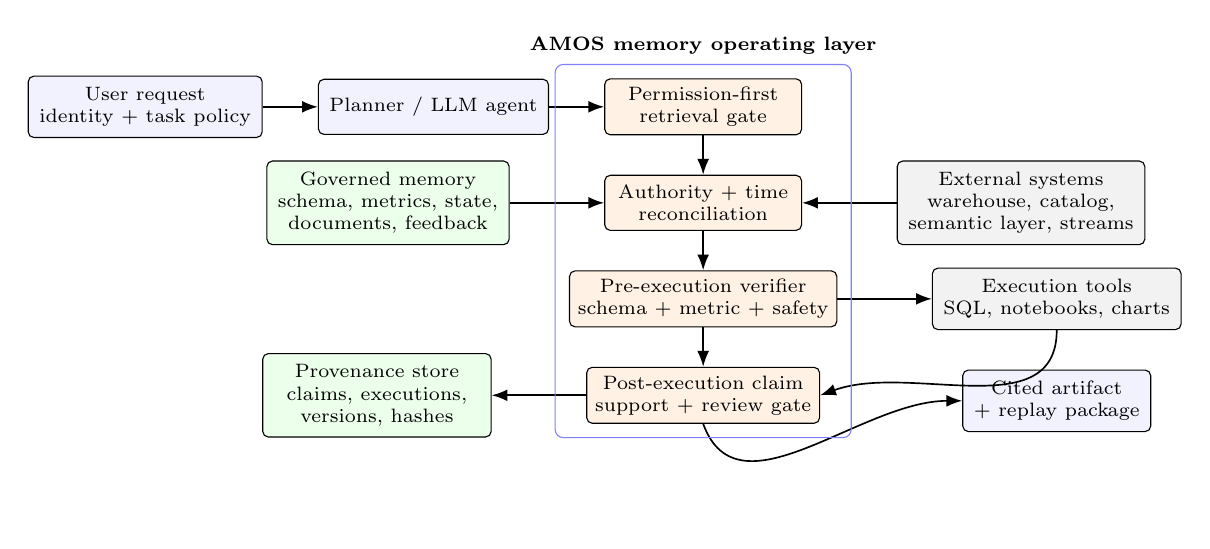
\begin{tikzpicture}[
  node distance=5mm and 7mm,
  every node/.style={font=\scriptsize, align=center},
  flow/.style={-Latex, semithick},
  box/.style={draw, rounded corners=2pt, fill=blue!5, minimum height=7mm, inner sep=4pt},
  gate/.style={draw, rounded corners=2pt, fill=orange!10, minimum width=25mm, minimum height=7mm, inner sep=3pt},
  store/.style={draw, rounded corners=2pt, fill=green!8, minimum width=29mm, inner sep=4pt},
  external/.style={draw, rounded corners=2pt, fill=gray!10, minimum width=31mm, inner sep=4pt}
]
\node[box] (request) {User request\\identity + task policy};
\node[box, right=of request] (agent) {Planner / LLM agent};
\node[gate, right=of agent] (permission) {Permission-first\\retrieval gate};
\node[gate, below=of permission] (reconcile) {Authority + time\\reconciliation};
\node[gate, below=of reconcile] (verify) {Pre-execution verifier\\schema + metric + safety};
\node[gate, below=of verify] (claimcheck) {Post-execution claim\\support + review gate};
\node[store, left=12mm of reconcile] (memory) {Governed memory\\schema, metrics, state,\\documents, feedback};
\node[store, left=12mm of claimcheck] (provenance) {Provenance store\\claims, executions,\\versions, hashes};
\node[external, right=12mm of reconcile] (systems) {External systems\\warehouse, catalog,\\semantic layer, streams};
\node[external, right=12mm of verify] (tools) {Execution tools\\SQL, notebooks, charts};
\node[box, below=of tools] (output) {Cited artifact\\+ replay package};

\draw[flow] (request) -- (agent);
\draw[flow] (agent) -- (permission);
\draw[flow] (permission) -- (reconcile);
\draw[flow] (reconcile) -- (verify);
\draw[flow] (verify) -- (claimcheck);
\draw[flow] (claimcheck.south) to[out=-70,in=180] (output.west);
\draw[flow] (memory) -- (reconcile);
\draw[flow] (systems) -- (reconcile);
\draw[flow] (verify) -- (tools);
\draw[flow] (tools.south) to[out=-90,in=20] (claimcheck.east);
\draw[flow] (claimcheck) -- (provenance);

\node[draw=blue!50, rounded corners=3pt, fit=(permission)(reconcile)(verify)(claimcheck), inner sep=5pt,
      label={[font=\scriptsize\bfseries]above:AMOS memory operating layer}] {};
\end{tikzpicture}
\caption{\amos as a memory operating layer. A bounded model-visible working set sits above persistent governed memory; permission filtering and reconciliation precede execution; verification and claim-support gates mediate tools and publication; provenance feeds later retrieval and replay.}
\label{fig:architecture}
\end{figure}

A minimal implementation requires bounded active context, persistent schema and semantic state, provenance memory, retrieval, verification, citation, and replay. Stream state, documents, prior analyses, and reviewer feedback extend the same operating interface without changing the agent-facing protocol.

\subsection{Memory Tiers}
\amos separates active context from persistent tiers for stream or snapshot state, schema/catalog metadata, semantic definitions, documents, prior analyses, feedback, and provenance; Appendix Table~\ref{tab:tiers} gives the detailed map.

\section{Memory Model and Operating Primitives}

\subsection{Memory Object}
A memory item is a typed object, not an arbitrary text chunk:

\begin{verbatim}
MemoryObject {
  id: stable identifier
  type: active_context | stream_state | schema | semantic_definition
        | document | prior_analysis | feedback | provenance
        | permission_policy
  content: structured metadata or an external-object reference
  summary: compact model-readable representation
  source: producing system or actor identifier
  authority: owner_approved | reviewer_approved | user_note
             | system_observed | model_hypothesis | untrusted_external
  effective_start, effective_end: interval described by the item
  transaction_time: time at which AMOS recorded the item
  permissions: required permission labels
  sensitivity: classification label
  version: source or policy version
  status: active | superseded | rejected | pending_review
  supersedes: identifiers replaced by this object
  provenance_ref: link to source object or producing computation
}
\end{verbatim}

The split between \code{effective\_time} and \code{transaction\_time} matters: a document may be recorded today but describe last quarter, and a reviewed metric may apply only to future reports.

\subsection{Runtime Invariants and Failure Semantics}
The proposed contract is defined by five publication invariants. Let $W_t$ be the model-visible working set, $E_t$ the executable computation, $Y_t$ the artifact, and $P_t$ the user's policy:
\begin{align}
I_1 &: \forall i \in W_t,\; permitted(i,P_t), \\
I_2 &: \forall i \in W_t,\; effective(i,t) \land \neg superseded(i,t), \\
I_3 &: execute(E_t) \Rightarrow schemaValid(E_t,W_t) \land metricValid(E_t,W_t) \land readOnly(E_t), \\
I_4 &: publish(Y_t) \Rightarrow \forall c \in importantClaims(Y_t),\; supported(c,\prov_t), \\
I_5 &: replayable(Y_t) \Rightarrow complete(R_t,W_t,E_t,\prov_t).
\end{align}
$I_1$ is enforced before model context construction; $I_2$ during retrieval and reconciliation; $I_3$ before tool execution; and $I_4$--$I_5$ before publication. These implications define the operating-layer boundary: sources and causal interpretations retain their own review requirements, while state validity and claim support become executable runtime properties.

The runtime returns one of five outcome classes. \code{reject} blocks execution or publication after an unresolved safety or validity failure. \code{repair} proposes a modified computation that must pass the same checks from the beginning. \code{warning} permits a mechanically valid artifact while exposing incomplete freshness or other bounded uncertainty. \code{needs\_review} keeps causal or operational claims non-final. \code{pass} means the configured structural checks succeeded.

The reference prototype uses snapshot consistency: each task records the memory IDs and external snapshot or offset references observed during the run. The deployment design pairs this record with atomic artifact/provenance publication, immutable source versions or leases, and invalidation when policy, schema, or metric state changes.

\subsection{Core Operating Primitives}
\amos exposes system-level primitives rather than prompting conventions: retrieve, write, supersede, reconcile, compact, verify, cite, and replay. These primitives form the stable agent-facing API while storage, retrieval, execution, and provenance backends can evolve independently. Appendix Table~\ref{tab:ops} defines their contracts.

\subsection{Runtime Protocol}
The runtime protocol starts with policy construction so inaccessible memory never enters model-visible context. \amos retrieves candidates, reconciles conflicts, builds a bounded working set, verifies tool calls, records execution, cites claims, and writes durable feedback only after verification gates run.

\begin{verbatim}
AMOS-RUN(q, user, policy, budget, provenance_level):
  task <- parse(q)
  candidates <- retrieve(task, policy, budget)
  working_set, conflicts <- reconcile(candidates)
  if unresolved(conflicts): return needs_review(conflicts)

  plan <- agent.plan(task, working_set)
  for step in plan.tool_steps:
      verify(step.sql_or_code, working_set, policy)
      result <- execute(step)
      record_execution(result)

  artifact <- agent.compose(task, working_set, results)
  claims <- extract_claims(artifact)
  for claim in claims:
      cite(claim, results, working_set, provenance_level)

  verification <- verify(artifact)
  replay_package <- package(task, plan, working_set, results,
                            verification)
  write(artifact, claims, provenance, replay_package)
  return artifact, verification, replay_package
\end{verbatim}

The ordering is the system contract: permission filtering precedes context injection, reconciliation precedes planning, verification precedes execution, provenance precedes publication, and memory writes preserve authority and review status. Deployments may replace individual steps with learned retrievers or richer verifiers.

\subsection{Retrieval and Reconciliation}
Retrieval combines semantic relevance with system constraints. The correctness-first prototype favors authority, effective time, supersession status, field-level matches, and permission filtering over raw lexical recall:
\begin{equation}
    score(i,q,t,u) = \alpha m(i,q) + \beta a(i) + \gamma f(i,t) + \delta v(i) + \eta s(i) - \lambda c(i,u),
\end{equation}
where $m$ is field-aware match quality, $a$ authority, $f$ freshness, $v$ verification/review status, $s$ active non-superseded status, and $c$ visible sensitivity risk. Access violations are filtered before scoring.

\begin{verbatim}
GOVERNED-RETRIEVE(q, user, time_range, budget):
  candidates <- lexical_candidates(q, candidate_budget)
  visible <- []
  for item in candidates:
      if not permitted(user, item.permissions):
          record_filtered(item)
          continue
      visible.append(item)

  scored <- []
  for item in visible:
      score <- field_match(q, item.id, item.type,
                           item.summary, item.content)
      score += authority_score(item.source, item.authority)
      score += freshness_score(item.effective_time, time_range)
      score += verification_score(item.status, item.review_state)
      score += supersession_score(item.status, item.supersedes)
      score -= sensitivity_penalty(item, user)
      scored.append((score, item))

  ranked <- sort_desc(scored)
  warnings <- ambiguity_warnings(ranked, q, time_range)
  return top_k(ranked, budget), warnings
\end{verbatim}

Ambiguity handling is part of the success criterion: when similarly named active items plausibly match, \amos surfaces a warning and keeps the approved task-relevant item near the top rather than silently accepting the first lexical match.

Conflict resolution follows a partial order, not blind recency. A default authority order is:
\begin{equation}
    owner\_approved > reviewer\_approved > user\_note > model\_hypothesis.
\end{equation}
Effective time constrains this order: a newer model hypothesis cannot override an older owner-approved definition that remains effective. Conflicting owner-approved definitions for the same interval are surfaced, not silently resolved.

\subsection{Stream-Aware but Not Stream-Only}
\amos is stream-aware, not stream-only. In batch settings, $M^s_t$ stores snapshot identifiers, table versions, query timestamps, partition ranges, and data-quality status rather than offsets and watermarks; the other tiers remain unchanged.

\section{Reference Implementation}

We implemented the memory operating layer as a deterministic reference system: SQL is template-selected, retrieved memory is typed, verification runs before execution, and artifacts are replayable from saved metadata. This isolates operating-layer behavior from variation in natural-language SQL generation.

The implementation uses SQLite FTS5/BM25 candidate generation followed by permission, temporal, authority, reconciliation, and reranking checks. Separate MiniLM/HNSW and reciprocal-rank-fusion paths evaluate how candidate generation affects the same governed protocol. The agent-facing operations remain unchanged across these backends.

\subsection{System Components}
The artifact uses SQLite for one-command reproduction. The schema separates memory objects, artifacts, claims, provenance edges, replay packages, and audit logs, with JSON payloads for versioned metadata. FTS5 triggers synchronize the lexical index with memory writes; source/target indexes support provenance lookup. Candidate-generation and storage backends change scale characteristics without changing the memory operating contract. Appendix Table~\ref{tab:prototype} summarizes the components.

\subsection{Synthetic Payment Scenario}
The prototype seeds 14{,}400 payment events over twelve hours. Failures rise in the final six-hour event-time window and concentrate in Processor B / Visa transactions. The dataset includes excluded test accounts, a deployment before the spike, late arrivals represented by watermark lag, and a schema migration from \code{failure\_reason} to \code{error\_code}. Seeded memory includes the approved \code{payment\_failure\_rate:v3} metric, current \code{payment\_events:v2} schema, stream state, a restricted prior incident, deployment evidence, reviewer feedback against over-attribution, and an analyst policy.

For the main request, the controller retrieves the approved metric, current schema, stream state, deployment note, reviewer feedback, and policy, while filtering the restricted incident for a user without \code{sre}. The report states that failure rate rose from 2.2\% to 7.4\%; Processor B / Visa reached 15.8\%. Deployment evidence remains review-gated rather than causal proof.

\subsection{Replay Package}
Each run writes a replay package with the request, plan, memory IDs, schema and metric versions, stream state, SQL, chart IDs, result hashes, and verifier status. Replay re-executes the saved SQL against DuckDB, regenerates the chart, and compares hashes, demonstrating that a continuous analytical artifact can carry the state required for audit and regeneration.

\section{Provenance, Verification, and Security}

\subsection{Claim-Level Provenance}
Artifact-level lineage is too coarse: one report may contain a correct chart, an outdated metric, and an unsupported causal explanation. \amos records provenance at the claim level:

\begin{verbatim}
ClaimProvenance {
  claim_id: sentence, chart annotation, slide bullet, or table cell
  artifact_id: report, notebook, chart, dashboard, or deck
  support: [query_id, notebook_cell_id, chart_id,
            document_ref, memory_object_id]
  data_state: [snapshot_id | stream_offset_range,
               watermark, event_time_window]
  semantic_state: [metric_definition_id, schema_version,
                   unit_definition]
  execution_state: [engine, runtime, parameters,
                    code_hash, result_hash]
  verification_state: [passed_checks, warnings,
                       unresolved_conflicts]
}
\end{verbatim}

This structure lets reviewers identify claims using superseded metrics, restricted sources, late-data-sensitive outputs, or expired replay state.

Figure~\ref{fig:claim-provenance} shows one concrete support graph. Edges are typed rather than generic citations: the numeric claim is computed by a query and chart, governed by metric and schema versions, scoped to a recorded data state, and checked by a verifier whose result enters the replay package.

\begin{figure}[H]
\centering
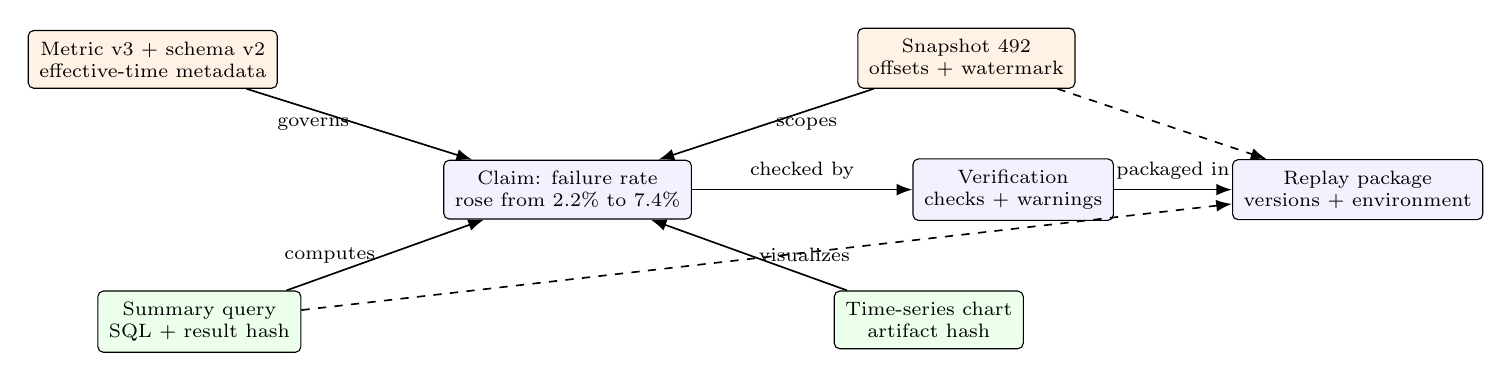
\begin{tikzpicture}[
  every node/.style={font=\scriptsize, align=center},
  item/.style={draw, rounded corners=2pt, fill=blue!5, inner sep=4pt},
  evidence/.style={draw, rounded corners=2pt, fill=green!8, inner sep=4pt},
  state/.style={draw, rounded corners=2pt, fill=orange!10, inner sep=4pt},
  edge/.style={-Latex, semithick, font=\tiny}
]
\node[item] (claim) {Claim: failure rate\\rose from 2.2\% to 7.4\%};
\node[evidence, below left=9mm and 18mm of claim] (query) {Summary query\\SQL + result hash};
\node[evidence, below right=9mm and 18mm of claim] (chart) {Time-series chart\\artifact hash};
\node[state, above left=9mm and 21mm of claim] (semantic) {Metric v3 + schema v2\\effective-time metadata};
\node[state, above right=9mm and 21mm of claim] (data) {Snapshot 492\\offsets + watermark};
\node[item, right=28mm of claim] (verification) {Verification\\checks + warnings};
\node[item, right=15mm of verification] (replay) {Replay package\\versions + environment};
\draw[edge] (query) -- node[left] {computes} (claim);
\draw[edge] (chart) -- node[right] {visualizes} (claim);
\draw[edge] (semantic) -- node[left] {governs} (claim);
\draw[edge] (data) -- node[right] {scopes} (claim);
\draw[edge] (claim) -- node[above] {checked by} (verification);
\draw[edge] (verification) -- node[above] {packaged in} (replay);
\draw[edge, dashed] (query) -- (replay);
\draw[edge, dashed] (data) -- (replay);
\end{tikzpicture}
\caption{Worked claim-level provenance graph. Support edges distinguish computation, semantic governance, data state, verification, and replay rather than attaching one artifact-level source list.}
\label{fig:claim-provenance}
\end{figure}

The prototype uses claim-type-specific support plans. Numeric rate claims cite summary/time-series queries and charts; concentration claims cite concentration queries; deployment and dashboard claims cite numeric, document, and approved-feedback evidence and remain review-gated. Coverage is complete only when support categories match the claim type.

\subsection{Provenance Levels}
Full replay is expensive and unnecessary for low-risk exploration. \amos therefore supports configurable provenance levels: high-risk reporting should use claim-level provenance or full replay; exploration may use artifact- or chart/query-level records. Appendix Table~\ref{tab:provlevels} lists the levels.

\subsection{Concrete Verifier}
Verification is structural and semantic, not a proof of truth. The prototype verifier rejects unsafe or stale computations before execution and downgrades unsupported interpretations after execution. It runs six checks.

\paragraph{SQL safety.} The parser must accept the query, and the root statement must be read-only. The verifier rejects writes, DDL, export/copy commands, and blocked raw columns such as \code{customer\_email}, \code{payment\_token}, or \code{raw\_payload}.

\paragraph{Schema validity.} SQL table and column references are compared with schema memory. For the current payment schema, \code{error\_code} is valid and superseded \code{failure\_reason} is rejected before execution.

\paragraph{Metric compliance.} The verifier checks the parsed SQL AST against the approved metric definition. For v3 of the payment-failure metric, the numerator must count \code{status = 'failure'} inside an aggregate, the denominator must include unfiltered attempts with \code{COUNT(*)}, and row filters must enforce production traffic, test-account exclusion, and an \code{event\_time} window. Equivalent predicates pass; comments or string literals do not.

\paragraph{Freshness and temporal state.} Artifacts must attach stream or snapshot state. The payment run records snapshot \code{payment\_events\_snapshot\_492}, interval 2026-07-07T14:00:00Z--20:00:00Z, offsets 125000--148999, watermark 19:58:30Z, and a 15-minute late-data policy. The 90-second watermark lag emits a warning.

\paragraph{Permission safety.} Retrieved memory is permission-checked before active-context construction. A user with \code{analytics,payments} receives aggregate payment memory and deployment evidence, not the prior incident requiring \code{sre}.

\paragraph{Provenance completeness and review obligations.} At level 3, numeric, causal, and recommendation claims must link to claim-appropriate queries, charts, metric/schema memory, data state, execution hashes, and verification status. Causal and operational claims also require document or approved-feedback evidence and remain \code{requires\_review} unless backed by an approved causal design.

The core controller emits explicit claim records from structured report templates. An additional extractor handles prose from reports, notebooks, and slides and is evaluated separately in Section~\ref{sec:extended-experiments}. Verification establishes compliance with encoded analytical and governance rules; causal interpretations remain review-gated.

\subsection{Security Model}
\amos treats retrieved content as untrusted. The security design uses five controls:
\begin{enumerate}
    \item \textbf{Permission-first retrieval:} inaccessible memory is filtered before model context construction.
    \item \textbf{Instruction/data separation:} retrieved text is labeled as evidence, not policy.
    \item \textbf{Tool sandboxing:} execution tools run with least-privilege credentials and auditable parameters.
    \item \textbf{Memory-write gates:} model-inferred memory remains low authority until reviewed.
    \item \textbf{Sensitive provenance handling:} provenance views are redacted according to user role and task need.
\end{enumerate}

The operating layer composes these controls with existing access control, secret isolation, execution sandboxes, audit logs, and organization-specific approval policies.

The seeded security suite covers indirect prompt injection, malicious prior analyses, malicious reviewer feedback, safe feedback rendering, provenance-link leakage, and cross-user filtering. \amos passes all six after adding authority-aware feedback ranking and separating low-authority evidence from applied reviewer guidance.

\section{Evaluation of Operating-Layer Correctness and Scale}

The evaluation tests whether the \amos memory operating layer enforces its contract across changing analytical state, preserves auditability, and maintains bounded agent context as persistent memory and provenance grow.

\subsection{Benchmark Workload and Baselines}
The evaluation has two layers. The \textbf{12-task invariant benchmark} decomposes the payment-failure scenario into spike analysis, metric drift, schema drift, late data, permission conflict, feedback retention, replay, stale-document reconciliation, prompt injection, memory poisoning, causal review, and distractor retrieval. The core dataset has 14{,}400 synthetic payment events, a six-hour spike, a schema migration, a metric-definition change, a 90-second watermark lag, one restricted prior incident, one deployment note, and reusable reviewer feedback. Retrieval probes add 5{,}000 distractor memory objects plus paraphrased, ambiguous, stale-similar, near-duplicate, and permission-dependent cases.

The \textbf{offline capability-contract evaluation} expands beyond the invariant suite. It runs fourteen local systems and adapters across payment failure, subscription churn, and warehouse quality, with twelve seeded variants and three deterministic repeats per domain. Variants inject dashboard pressure, wording paraphrases, late-data probes, prompt-injection documents, restricted-incident traps, schema-rename traps, and stale-metric traps. Full-contract pass requires analytical correctness, permission safety, the review boundary, claim provenance, and replay; metric-axis tables report partial capability separately.

On the invariant benchmark we compare five local baselines. \textbf{Metadata-filtered RAG} calls the local retriever with access-control and status filtering but lacks metric/schema verification and replay. \textbf{Semantic-layer agent} validates approved metrics but lacks schema, stream-state, provenance, and permission gates. \textbf{Catalog+lineage+dbt agent} uses schema, metric, stream-state, and permission checks, but lacks claim-level citation and feedback memory. \textbf{Strong long context} serializes memory broadly without pre-context permission filtering, authority reconciliation, or replay. \textbf{Structured tool-using LLM agent} remains a deterministic offline simulation in the invariant table for repeatability; the live-model pilot is reported separately.

The capability analysis adds the same families plus two \textbf{strong local baselines} (manual policy-prompt agent and permission-filtered RAG) that receive current metric/schema context and permission filtering; three \textbf{OSS-shaped adapters} that load exported-interface fixtures (SQLite FTS5 RAG documents, MetricFlow/dbt-metrics JSON, and OpenLineage-shaped events); and three \textbf{component ablations} that disable the verifier, permission gate, or provenance recorder one at a time.

\subsection{Task Protocol}
Each task is an input request plus a seeded memory/data perturbation. The predefined success criterion is structural: required SQL predicates, memory versions, permission exclusions, claim-specific provenance links, and final status. For example, metric drift passes when the AST-backed verifier rejects or repairs a query that omits test-account exclusion; causal review passes when deployment and dashboard claims are marked \code{needs\_review}. Table~\ref{tab:task-protocol} summarizes the protocol.

\begin{table}[t]
\centering
\scriptsize
\setlength{\tabcolsep}{3pt}
\begin{tabular}{L{0.20\linewidth}L{0.24\linewidth}L{0.28\linewidth}L{0.18\linewidth}}
\toprule
\textbf{Task family} & \textbf{Perturbation} & \textbf{Expected evidence or decision} & \textbf{Gate} \\
\midrule
Metric/schema drift & Superseded metric or column is salient. & Uses metric v3/schema v2; rejects stale SQL before execution. & Verifier \\
Late data & Watermark trails the interval by 90 seconds. & Records offsets and watermark; emits freshness warning. & Stream-state check \\
Permission conflict & Relevant prior incident is restricted. & Excludes restricted memory from context and citations. & Retrieval gate \\
Feedback retention & Reviewer correction is written once. & Later task retrieves correction and avoids over-attribution. & Memory write/retrieve \\
Replay/provenance & Saved artifact is regenerated. & SQL hashes, chart metadata, memory IDs, and verification state match. & Replay engine \\
Adversarial memory & Injection text or low-authority metric is retrieved. & Treats text as data; approved memory prevails. & Reconciliation/write gate \\
Causal review & Deployment note precedes spike. & Marks causal and dashboard-update claims \code{needs\_review}. & Claim verifier \\
Distractor retrieval & 5{,}000 unrelated memories are added. & Approved metric remains rank 1. & Retriever \\
\bottomrule
\end{tabular}
\caption{Task protocol. The benchmark scores the expected system decision, including warnings, rejections, and \code{needs\_review} outcomes, rather than rewarding only complete answers.}
\label{tab:task-protocol}
\end{table}

Baselines receive the seeded metadata their capability would normally consume. They fail only when their local policy lacks an operation required by the criterion, such as durable feedback memory, claim-level replay, or pre-context instruction/data separation.

Reported \amos invariant-benchmark runtime is averaged over three deterministic local runs. The extended harness adds local baseline policies, noisy retrieval variants, a 50-case invariant regression suite, a frozen verifier engineering corpus, a 1{,}000-example claim-extraction corpus, seeded security probes, 5{,}000-distractor retrieval, and concurrent retrieval measurements. Capability-contract executions use the deterministic offline live-agent provider and record per-run contracts, metric axes, failures, and provenance-overhead pairs.

\subsection{Metrics}
The primary outcomes are state correctness, bounded-context governance, auditability, replay, retrieval quality, update visibility, and indexed scaling behavior. Appendix Table~\ref{tab:metrics} defines the metric set used by the harness.

\subsection{Benchmark Results}
Table~\ref{tab:prototype-results} reports aggregate criterion matches. \amos matches all 12 outcomes, including non-final warning, rejection, downgrade, and \code{needs\_review} decisions. The strongest baseline, catalog+lineage+dbt, matches 6 of 12: it handles schema, metric, late-data, permission, memory-poisoning, and retrieval-stress checks, but fails integrated spike analysis, feedback retention, replay, stale-document reconciliation, prompt-injection isolation, and causal-review obligations. The offline structured-LLM baseline passes only schema syntax.

\begin{table}[t]
\centering
\scriptsize
\setlength{\tabcolsep}{3pt}
\begin{tabular}{L{0.34\linewidth}C{0.12\linewidth}C{0.12\linewidth}C{0.12\linewidth}C{0.12\linewidth}}
\toprule
\textbf{System} & \textbf{Matches} & \textbf{Tasks} & \textbf{Rate} & \textbf{Mean runtime} \\
\midrule
\textbf{\amos} & \textbf{12} & \textbf{12} & \textbf{1.000} & \textbf{0.268 s} \\
Catalog+lineage+dbt agent & 6 & 12 & 0.500 & \na \\
Metadata-filtered RAG & 3 & 12 & 0.250 & \na \\
Semantic-layer agent & 3 & 12 & 0.250 & \na \\
Strong long context & 3 & 12 & 0.250 & \na \\
Structured tool-using LLM & 1 & 12 & 0.083 & \na \\
\bottomrule
\end{tabular}
\caption{Aggregate results over the 12-task benchmark. A match means the system produced the expected decision, including \code{warning}, \code{reject}, or \code{needs\_review} where required. \amos runtime is averaged over three local analysis runs; baseline timings are omitted because the baselines are component policies rather than comparable end-to-end systems.}
\label{tab:prototype-results}
\end{table}

\amos returns a warning for the integrated report because the watermark lags the requested window and causal/dashboard claims require review. The artifact remains replayable and cited, while tentative causality is not presented as final.

\subsection{Task-Level Results}
Appendix Table~\ref{tab:scenario-checks} gives task-level results for selected baselines. The \amos status is the observed system decision, not just a binary success label.

\subsection{Multi-Domain Capability-Contract Evaluation}
Table~\ref{tab:product-eval} summarizes full-contract outcomes. Across payment failure, subscription churn, and warehouse quality, \amos passes all twelve seeded variants in all three deterministic repeats per domain. The all-or-nothing result is reported with metric-axis scores so analytical capability can be distinguished from operating-layer provenance and replay coverage.

\begin{table}[t]
\centering
\scriptsize
\setlength{\tabcolsep}{3pt}
\begin{tabular}{L{0.28\linewidth}C{0.14\linewidth}C{0.14\linewidth}C{0.14\linewidth}C{0.14\linewidth}}
\toprule
\textbf{System} & \textbf{Payment} & \textbf{Churn} & \textbf{Warehouse} & \textbf{Provenance / replay} \\
\midrule
\textbf{\amos} & \textbf{12/12} & \textbf{12/12} & \textbf{12/12} & \textbf{1.0 / 1.0} \\
Strong baselines (policy prompt; RAG+perm) & 0/12 & 0/12 & 0/12 & 0.0 / 0.0 \\
OSS-shaped adapters (FTS5 RAG; metrics JSON; OpenLineage) & 0/12 & 0/12 & 0/12 & 0.0 / 0.0 \\
Simple RAG / semantic / catalog / long context / agent-only & 0/12 & 0/12 & 0/12 & 0.0 / 0.0 \\
\amos no verifier & 0/12 & 3/12 & 0/12 & 1.0 / 0.5--0.75 \\
\amos no permission gate & 0/12 & 0/12 & 0/12 & 1.0 / 1.0 \\
\amos no provenance & 0/12 & 0/12 & 0/12 & 0.0 / 1.0 \\
\bottomrule
\end{tabular}
\caption{Offline capability-contract matches by seeded variant; each variant is repeated deterministically three times. A variant passes when all repeats satisfy task correctness, permission safety, review boundary, claim provenance, and replay.}
\label{tab:product-eval}
\end{table}

The metric-axis breakdown clarifies the comparator story (Appendix Table~\ref{tab:metric-axes}). In the payment domain, both strong baselines and the OSS semantic/catalog adapters score 1.0 on task, SQL, metric, schema, permission, and review axes, yet 0.0 on provenance and replay. The OSS FTS5 RAG adapter reaches 0.75 on the analytical axes with permission safety 1.0. Catalog and semantic legacy baselines can ground SQL and metrics without satisfying the full memory contract. Ablations confirm complementary failure modes: disabling the permission gate collapses permission safety while preserving provenance and replay; disabling provenance recording preserves analytical axes and replay but fails claim support; disabling the verifier damages SQL/metric/schema compliance and reduces replay success.

Matched provenance-overhead executions hold provider, prompts, SQL/tool path, verifier, and replay constant while disabling claim recording. After repeats are collapsed by seeded variant, the payment-domain mean latency delta is about 0.047\,s and the measured raw-evidence delta is about 198 bytes.

Scenario-pack manifests cover three domains with capability-evaluation and live-agent adapters; 120 generated cross-domain task variants pass manifest-contract checks. The scored tables use the twelve executed variants per domain.

\subsection{Ablations and Large-Scale Memory Behavior}
Appendix Table~\ref{tab:ablations} reports ablations on the 12-task invariant benchmark. Removing the verifier drops five tasks; removing stream/snapshot memory or semantic memory drops three each.

We replaced full-store scans with FTS5/BM25 candidate generation and reran one fixed local protocol at 10{,}001, 100{,}001, and 1{,}000{,}001 total memories, paired with 10{,}000, 100{,}000, and 1{,}000{,}000 provenance edges. The approved metric remains rank 1 in 30/30, 30/30, and 20/20 serial retrievals. Serial p50 latency rises from 0.045\,s to 0.145\,s and 4.997\,s; p95 rises from 0.047\,s to 0.152\,s and 8.488\,s. At eight readers, p95 is 0.411\,s, 0.717\,s, and 4.548\,s. All runs keep the FTS row count synchronized, observe permission revocation and metric supersession, and complete their mixed read/write workload without recorded errors. The million-scale database occupies about 1.50\,GB after all probes. Figure~\ref{fig:scale-latency} shows the latency curve.

\begin{figure}[H]
\centering
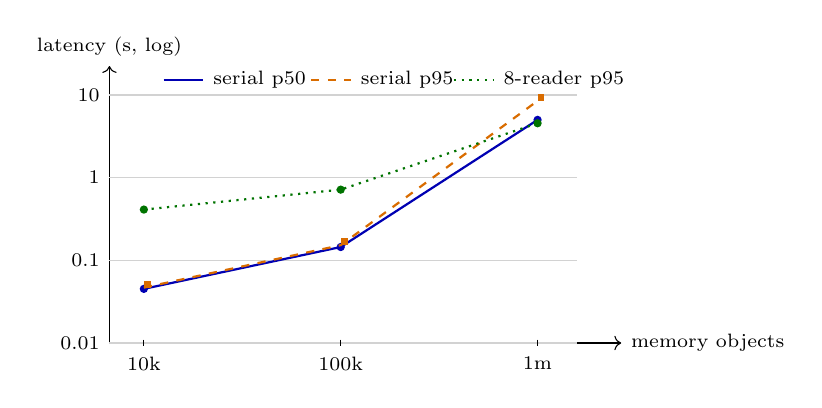
\begin{tikzpicture}[x=1.25cm,y=1.05cm,font=\scriptsize]
  \draw[->] (0,0) -- (5.2,0) node[right] {memory objects};
  \draw[->] (0,0) -- (0,3.35) node[above] {latency (s, log)};
  \foreach \y/\label in {0/{0.01},1/{0.1},2/{1},3/{10}} {
    \draw[gray!35] (0,\y) -- (4.75,\y);
    \node[left] at (0,\y) {\label};
  }
  \foreach \x/\label in {0.35/{10k},2.35/{100k},4.35/{1m}} {
    \draw (\x,0.04) -- (\x,-0.04);
    \node[below] at (\x,-0.05) {\label};
  }
  \draw[blue!70!black,thick] plot coordinates {(0.35,0.655) (2.35,1.161) (4.35,2.699)};
  \foreach \x/\y in {0.35/0.655,2.35/1.161,4.35/2.699} \fill[blue!70!black] (\x,\y) circle (1.5pt);
  \draw[orange!85!black,thick,dashed] plot coordinates {(0.35,0.670) (2.35,1.183) (4.35,2.929)};
  \foreach \x/\y in {0.35/0.670,2.35/1.183,4.35/2.929} \fill[orange!85!black] (\x,\y) rectangle +(2.5pt,2.5pt);
  \draw[green!45!black,thick,dotted] plot coordinates {(0.35,1.614) (2.35,1.855) (4.35,2.658)};
  \foreach \x/\y in {0.35/1.614,2.35/1.855,4.35/2.658} \fill[green!45!black] (\x,\y) circle (1.5pt);
  \draw[blue!70!black,thick] (0.55,3.18) -- (0.95,3.18) node[right,black] {serial p50};
  \draw[orange!85!black,thick,dashed] (2.05,3.18) -- (2.45,3.18) node[right,black] {serial p95};
  \draw[green!45!black,thick,dotted] (3.50,3.18) -- (3.90,3.18) node[right,black] {8-reader p95};
\end{tikzpicture}
\caption{Single-machine indexed memory retrieval. The model-visible working set remains bounded while persistent state grows from 10k to one million objects; rank-1 correctness holds at every scale and the curve quantifies backend tail latency.}
\label{fig:scale-latency}
\end{figure}

Provenance insertion throughput is about 109k edges/s at 10k edges, 73k at 100k, and 44k at one million. Indexed target-query p95 is 0.0009\,s, 0.0027\,s, and 0.273\,s, respectively. Together with memory retrieval, these measurements demonstrate the operating-layer separation: analytical history scales outside the prompt, while the agent consumes a fixed-budget working set. Candidate generation and million-object tail latency become backend optimization targets rather than changes to the agent protocol.

\subsection{Governed Lexical, Vector, and Hybrid Retrieval}
We separately compare three candidate-generation paths while holding the post-retrieval operating contract fixed: SQLite FTS5/BM25 plus governed reranking; cosine HNSW over pinned MiniLM-L6-v2 embeddings (revision prefix \code{1110a243fdf4}, $M=16$, \code{ef\_construction=200}, search \code{ef=128}); and reciprocal-rank fusion ($k=60$). The bundle records the full model identifier and revision hash. The controlled workload contains twelve target metrics, 24 lexical or semantic-paraphrase queries, restricted and superseded near-duplicates, and templated distractors. Table~\ref{tab:retrieval-engines} reports the frozen results at 1k, 10k, and 100k distractors.

\begin{table}[H]
\centering
\scriptsize
\setlength{\tabcolsep}{2.5pt}
\begin{tabular}{C{0.08\linewidth}C{0.12\linewidth}C{0.12\linewidth}C{0.14\linewidth}C{0.12\linewidth}C{0.13\linewidth}C{0.12\linewidth}}
\toprule
\textbf{Distr.} & \textbf{BM25 top-1} & \textbf{BM25 p95} & \textbf{HNSW top-1} & \textbf{HNSW p95} & \textbf{Hybrid R@5} & \textbf{Hybrid p95} \\
\midrule
1k & 0.667 & 0.267\,s & 0.917 & 0.013\,s & 0.917 & 0.283\,s \\
10k & 0.667 & 2.036\,s & 0.708 & 0.016\,s & 0.875 & 1.860\,s \\
100k & 0.667 & 17.326\,s & 0.208 & 0.030\,s & 0.833 & 16.746\,s \\
\bottomrule
\end{tabular}
\caption{Governed retrieval-engine comparison. HNSW query latency stays low, but fixed-configuration relevance collapses in duplicated semantic neighborhoods at 100k. Hybrid retrieval preserves broader recall while inheriting the lexical full-store fallback tail. Across all engines and scales, permission-leak and superseded-item-leak counts are zero.}
\label{tab:retrieval-engines}
\end{table}

MiniLM/HNSW is strongest at 1k but loses relevance as duplicated semantic neighborhoods crowd the fixed index; hybrid retrieval recovers recall while inheriting the lexical tail. Permission-revocation and metric-supersession probes pass at every archived scale. At 100k, SQLite/FTS5 seeding and indexing takes approximately 6.8\,s and 70\,MB, whereas embedding plus HNSW construction takes approximately 667\,s and 169\,MB. The result motivates adaptive candidate generation beneath the same operating layer: vector search for latency, lexical evidence for recall, and governance checks after fusion.

\subsection{Extended Operating-Layer Experiments}\label{sec:extended-experiments}
The extended harness covers verifier regressions, retrieval ambiguity, invariant variants, scaled claim extraction, seeded security attacks, OSS-shaped adapter probes, and concurrency. Appendix Table~\ref{tab:extended-results} summarizes the results.

Noisy retrieval and security probes exposed failures in the earlier keyword-only retriever and report renderer. The revised retriever adds field-aware matching, authority-aware feedback ranking, supersession-aware scoring, and ambiguity warnings; the report generator separates approved feedback from low-authority evidence. Canonical, paraphrased, stale-similar, and permission-dependent probes rank the approved metric first; the ambiguous metric-name probe warns and keeps it in the top two.

Claim extraction is evaluated on a 1{,}000-example seed-controlled corpus spanning report, notebook, slide, ambiguous, subscription, and warehouse artifacts. A regex/keyword extractor reaches mean type precision 0.958, recall 1.0, and review-obligation recall 1.0.

The artifact also includes versioned intake contracts for independent holdout tasks and real claim annotations. Validators hash sealed references, enforce author/reviewer/annotator/adjudicator separation, prevent source-group leakage across splits, preserve pre-adjudication labels, verify exact annotation spans, and align task IDs before paired analysis. This creates a reproducible path from controlled operating-layer tests to independent external evaluation.

After replacing flat column-name checks with scoped SQL qualification, a frozen 16-case regression corpus accepts all six labeled-valid queries and rejects all ten labeled-invalid queries. Cases cover aliases, CTE outputs, conditional aggregates, stale and unknown columns, blocked columns, missing metric filters, wrong time fields, adversarial text, and writes.

The archived live feasibility pilot uses the authenticated OpenAI Codex CLI with model \code{gpt-5.6-sol}. A strict lexical grader marks 3 of 8 policy responses as passing, while all three corrected-verifier end-to-end tasks complete with the expected \code{warning} status for watermark lag and review-gated causal claims. One SQL-proposal call times out at 180 seconds; its raw trace is preserved and the isolated retry completes, yielding 3/3 end-to-end completions and zero unresolved provider failures.

\subsection{Evaluation Scope and External Protocol}
The reported results are controlled reference-system evidence: deterministic task variants measure contract enforcement, fixed system studies measure indexed state growth, and the live pilot checks end-to-end feasibility. We therefore report exact task counts and fixed-workload measurements rather than population estimates. A frozen external protocol extends this foundation with 150 independently authored tasks across three domains, multiple model families and prompt frames, double-annotated real artifacts, red-team testing, a reviewer audit study, and a production-faithful comparison system. Separation of task authors, annotators, adjudicators, and system developers is enforced by executable intake validators.

\section{Discussion and Systems Roadmap}

\subsection{Why an Operating Layer?}
RAG retrieves evidence; catalogs describe assets and governance metadata; semantic layers define metrics; lineage systems track datasets, jobs, and runs. \amos does not replace these systems. It treats them as memory sources and execution references, while adding runtime control of the agent's evolving analytical working state.

The distinction is operational. RAG can retrieve a metric document without deciding whether its version is effective for the requested interval. A catalog can expose a column without ensuring that a report used the valid schema version. A semantic layer can define \code{payment\_failure\_rate} without attaching it to every textual claim. A lineage tool can record a table read without carrying a reviewer correction into the next task. \amos supplies the shared layer above them: retrieve bounded context, check temporal validity and permissions, reconcile conflicts, execute tools, verify outputs, attach claim-level provenance, replay prior work, and persist corrections.

\subsection{Large-Scale Deployment Model}
The operating layer is risk-adaptive. Exploratory analysis can use artifact-level records, while executive or regulated reporting can require claim-level support and full replay. In the matched payment workload, claim recording adds about 0.047\,s mean latency and 198 bytes to measured raw evidence. Persistent state is indexed outside the model, and the active-context budget remains fixed; compaction, retention, invalidation, and storage backends can therefore be tuned without changing the agent-facing API.

The integration path is direct: catalogs and semantic layers populate authoritative memory; warehouse snapshots and stream processors provide data-state references; execution engines provide code and result hashes; and lineage systems receive the resulting claim graph. The systems roadmap advances this composition through distributed metadata storage, adaptive hybrid retrieval, policy churn, concurrent execution, and connectors for dbt, OpenLineage, DataHub/OpenMetadata, warehouse snapshot APIs, and orchestration logs.

\section{Conclusion}

Continuous large-scale data analysis agents need more than stronger models, larger prompts, or better SQL generation. They need a memory operating layer that manages schemas, semantic definitions, stream or snapshot state, prior analyses, review feedback, permissions, execution history, and provenance as first-class resources. \amos defines that abstraction and implements it as a bounded-context protocol over persistent, typed analytical state.

The central result is that continuous analysis is memory-bound as well as model-bound. Agents must know which context is valid, which definitions are authoritative, which data state was used, which claims are supported, and which corrections persist. \amos turns these requirements into operating-layer invariants. It satisfies the full contract across the invariant benchmark and three analytical domains, preserves permission and supersession controls across retrieval engines, and records replayable claim support while indexed state reaches one million memory objects and one million provenance edges. This establishes a concrete systems foundation for agents that continuously analyze large and changing data environments without allowing prompt context to become the system of record.

\appendix
\section{Detailed Tables}
\setcounter{table}{0}
\renewcommand{\thetable}{A\arabic{table}}
\renewcommand{\theHtable}{A\arabic{table}}

\begin{table}[p]
\centering
\small
\begin{tabular}{L{0.22\linewidth}L{0.35\linewidth}L{0.33\linewidth}}
\toprule
\textbf{Failure mode} & \textbf{Risk} & \textbf{\amos control} \\
\midrule
Temporal staleness & Answer uses an expired definition or data state. & Effective-time and supersession checks. \\
Schema drift & Query references a removed or renamed column. & Schema-version validation before execution. \\
Metric drift & A metric means different things across teams or dates. & Authoritative semantic memory with effective dates. \\
Late data & Result ignores events arriving after the first watermark. & Recorded offsets, watermarks, and late-data policy. \\
Feedback loss & Reviewer correction is not applied later. & Durable feedback memory and retrieval constraints. \\
Unsupported claim & Report states a cause without support. & Claim-level provenance and citation checks. \\
Unauthorized retrieval & Agent uses restricted data or documents. & Permission filtering before context injection and tool execution. \\
Prompt injection & Retrieved text issues malicious instructions. & Instruction/data separation, sandboxed tools, and write gates. \\
\bottomrule
\end{tabular}
\caption{Representative analytical-agent failure modes and the \amos controls that make them inspectable.}
\label{tab:failures}
\end{table}

\begin{table}[p]
\centering
\small
\begin{tabular}{L{0.19\linewidth}L{0.35\linewidth}L{0.35\linewidth}}
\toprule
\textbf{Tier} & \textbf{Stores} & \textbf{Used for} \\
\midrule
Active context & Current task, selected definitions, schema, and recent tool results. & Model-visible working set. \\
Stream/snapshot state & Offsets, watermarks, event windows, snapshot IDs, late-data policy. & Temporal validity and replay. \\
Schema/catalog & Tables, columns, joins, owners, sensitivity labels, schema versions. & Query grounding and permissions. \\
Semantic definitions & Metrics, rules, units, dimensions, effective dates, owners. & Consistent meaning across analyses. \\
Documents & Runbooks, incident reports, requirements, design notes, summaries. & Source-backed context treated as evidence. \\
Prior analyses & Accepted SQL, notebooks, charts, explanations, dashboard notes. & Reuse work and preserve analytical history. \\
Feedback & Corrections, rejected assumptions, approvals, escalation notes. & Durable human review. \\
Provenance & Claim-query, query-data, artifact-memory, and version links. & Auditability, impact analysis, and replay. \\
\bottomrule
\end{tabular}
\caption{Typed memory tiers managed by \amos.}
\label{tab:tiers}
\end{table}

\begin{table}[p]
\centering
\small
\begin{tabular}{L{0.24\linewidth}L{0.66\linewidth}}
\toprule
\textbf{Operation} & \textbf{Contract} \\
\midrule
\code{retrieve(q, policy)} & Return a bounded, permissioned, temporally valid working set. \\
\code{write(item)} & Persist memory with source, authority, time, permissions, and provenance. \\
\code{supersede(old,new)} & Replace an item while preserving lineage. \\
\code{reconcile(items)} & Resolve conflicts by authority, effective time, review status, and source type; surface unresolved conflicts. \\
\code{compact(items)} & Shrink memory while preserving provenance and validity metadata. \\
\code{verify(artifact)} & Check schema, metrics, freshness, permissions, execution status, and provenance coverage. \\
\code{cite(claim)} & Link a claim to supporting data, code, definitions, memory, and verification results. \\
\code{replay(artifact)} & Re-execute or audit using recorded snapshots, offsets, code, and memory versions. \\
\bottomrule
\end{tabular}
\caption{Core \amos memory operations.}
\label{tab:ops}
\end{table}

\begin{table}[p]
\centering
\small
\begin{tabular}{L{0.23\linewidth}L{0.34\linewidth}L{0.33\linewidth}}
\toprule
\textbf{Role} & \textbf{Local implementation} & \textbf{Production role} \\
\midrule
Memory/provenance store & SQLite tables for memory, artifacts, claims, provenance edges, replay packages, and audit logs. & Durable governed state; production could use PostgreSQL/JSONB/pgvector. \\
SQL engine & DuckDB over synthetic payment events. & Read-only analytical execution and deterministic result-hash replay. \\
Notebook-style runner & Python controller for parse, retrieve, plan, verify, query, chart, report, cite, and package. & Ordered, testable execution similar to notebook cells. \\
LLM-agent harness & Offline provider plus OpenAI Responses and authenticated ephemeral Codex CLI transports. & Preserves raw prompts, outputs, model identity, latency, token totals, verifier failures, and repairs. \\
Verifier & Rule checks over SQL ASTs, schema, metrics, stream state, policy, and claims. & Rejects invalid computation and marks unsupported claims for review. \\
Artifact store & Filesystem Markdown, SQL, PNG, JSON provenance, and replay files. & Inspectable reports, charts, queries, and replay metadata. \\
\bottomrule
\end{tabular}
\caption{Reference implementation components and their corresponding deployment roles beneath the memory operating layer.}
\label{tab:prototype}
\end{table}

\begin{table}[p]
\centering
\small
\begin{tabular}{C{0.10\linewidth}L{0.50\linewidth}L{0.30\linewidth}}
\toprule
\textbf{Level} & \textbf{Recorded support} & \textbf{Typical use} \\
\midrule
0 & No durable provenance. & Disposable exploration. \\
1 & Artifact-level inputs and tools. & Low-risk reports or notebooks. \\
2 & Chart/query links to source computations. & Reused charts and SQL outputs. \\
3 & Claim links to computations, definitions, data state, and memory versions. & High-risk reporting. \\
4 & Full replay package: code, parameters, snapshots/offsets, memory versions, and environment metadata. & Audits and regulated workflows. \\
\bottomrule
\end{tabular}
\caption{Configurable provenance levels. Higher-risk artifacts should use claim-level provenance or full replay.}
\label{tab:provlevels}
\end{table}

\begin{table}[p]
\centering
\small
\begin{tabular}{L{0.25\linewidth}L{0.62\linewidth}}
\toprule
\textbf{Metric} & \textbf{What it checks} \\
\midrule
Task correctness & Final answer, SQL, chart, or report matches the predefined criterion. \\
Temporal correctness & Result uses the correct snapshot, offsets, watermark, and effective definitions. \\
Metric correctness & Query obeys the approved metric definition, filters, and time field. \\
Schema correctness & SQL is compatible with the active schema version. \\
Provenance coverage & Important claims link to required computation, data state, definitions, and memory versions. \\
Replay success & Saved SQL, hashes, chart metadata, and memory versions regenerate the artifact. \\
Feedback retention & Reviewer corrections are written to memory and retrieved later. \\
Permission safety & Restricted memory is filtered before active-context construction. \\
Overhead & Added local runtime for retrieval, verification, provenance recording, and replay packaging. \\
\bottomrule
\end{tabular}
\caption{Evaluation metrics for a continuous large-scale analytical memory operating layer.}
\label{tab:metrics}
\end{table}

\begin{table}[p]
\centering
\scriptsize
\setlength{\tabcolsep}{3pt}
\begin{tabular}{L{0.30\linewidth}L{0.14\linewidth}C{0.13\linewidth}C{0.13\linewidth}C{0.13\linewidth}}
\toprule
\textbf{Task} & \textbf{\amos decision} & \textbf{Catalog+ lineage} & \textbf{Metadata RAG} & \textbf{Long context} \\
\midrule
Payment spike & Warning & \fail & \fail & \fail \\
Metric drift & Repaired & \pass & \fail & \pass \\
Schema drift & Reject stale SQL & \pass & \fail & \pass \\
Late data & Warning & \pass & \fail & \fail \\
Permission conflict & Filtered & \pass & \pass & \fail \\
Feedback retention & \pass & \fail & \fail & \pass \\
Provenance replay & \pass & \fail & \fail & \fail \\
Stale document & Reconciled & \fail & \pass & \fail \\
Prompt injection & Isolated & \fail & \fail & \fail \\
Memory poisoning & Downgraded & \pass & \fail & \fail \\
Causal review & \code{needs\_review} & \fail & \fail & \fail \\
Retrieval stress & \pass & \pass & \pass & \fail \\
\bottomrule
\end{tabular}
\caption{Task-level results for selected baselines. \amos decisions such as warning, downgrade, rejection, and \code{needs\_review} count as matches only when the task expects that non-final decision.}
\label{tab:scenario-checks}
\end{table}

\begin{table}[p]
\centering
\small
\begin{tabular}{L{0.30\linewidth}C{0.15\linewidth}L{0.43\linewidth}}
\toprule
\textbf{Removed component} & \textbf{Pass rate} & \textbf{Newly failing tasks} \\
\midrule
Verifier & 0.583 & schema drift, metric drift, late data, causal review, memory poisoning \\
Stream/snapshot memory & 0.750 & late data, provenance replay, integrated spike task \\
Semantic memory & 0.750 & metric drift, integrated spike task, memory poisoning \\
Schema/catalog memory & 0.833 & schema drift, integrated spike task \\
Provenance memory & 0.833 & provenance replay, causal review \\
Feedback memory & 0.917 & feedback retention \\
Permission filter & 0.917 & permission conflict \\
\bottomrule
\end{tabular}
\caption{Ablation probes over the 12-task benchmark. Pass rates are computed after forcing the listed invariants to fail when the supporting component is removed.}
\label{tab:ablations}
\end{table}

\begin{table}[p]
\centering
\scriptsize
\setlength{\tabcolsep}{3pt}
\begin{tabular}{L{0.27\linewidth}L{0.21\linewidth}L{0.42\linewidth}}
\toprule
\textbf{Probe} & \textbf{Result} & \textbf{Takeaway} \\
\midrule
Implemented local baselines & Strongest baseline 6/12; RAG, semantic layer, and long context 3/12. & Executable policy implementations replace hand scoring and expose capability-level differences. \\
Noisy retrieval variants & 5/5 under ambiguity-aware criteria. & Approved metric ranks first except the ambiguous-name case, which warns and keeps it top two. \\
Invariant variants & 50/50 pass rate. & Covers SQL predicate variants, missing metric filters, stale columns, permission changes, and malicious feedback authority. \\
Free-form claim extraction & 1{,}000-example corpus; precision 0.958, recall 1.0, review recall 1.0. & Covers report, notebook, slide, ambiguous, subscription, and warehouse templates. \\
Seeded security suite & 6/6 pass rate. & Cross-user filtering, prompt injection, malicious analyses/feedback, safe rendering, and provenance-link leakage pass locally. \\
Indexed scale and concurrency & 10k/100k/1m distractors: rank 1 in all 80 serial runs; p95 0.047/0.152/8.488s. & Quantifies candidate-generation and tail-latency behavior across three orders of magnitude. \\
Live LLM feasibility pilot & Policy rubric 3/8; corrected-verifier end-to-end 3/3 graded; archive status completed. & Preserves the timeout trace and successful isolated retry for end-to-end auditability. \\
Verifier engineering corpus & 6/6 labeled-valid accepted; 10/10 labeled-invalid rejected. & Frozen regression coverage for aliases, CTEs, metric rules, schema, permissions, and writes. \\
OSS-shaped adapters & Payment semantic/catalog task axes 1.0; FTS5 RAG 0.75; full-contract 0/12 variants. & Export-shaped RAG/semantic/OpenLineage adapters close analytical gaps but not provenance/replay. \\
Offline capability analysis (3 domains) & \amos 12/12 seeded variants per domain; strong/OSS adapters 0/12. & Each variant has three deterministic repeats and complete metric-axis traces. \\
\bottomrule
\end{tabular}
\caption{Extended memory-operating-layer experiments covering correctness, safety, extraction, adapters, and scale.}
\label{tab:extended-results}
\end{table}

\begin{table}[p]
\centering
\scriptsize
\setlength{\tabcolsep}{2.2pt}
\begin{tabular}{L{0.24\linewidth}C{0.08\linewidth}C{0.08\linewidth}C{0.08\linewidth}C{0.08\linewidth}C{0.09\linewidth}C{0.09\linewidth}C{0.08\linewidth}C{0.08\linewidth}}
\toprule
\textbf{System} & \textbf{Task} & \textbf{SQL} & \textbf{Metric} & \textbf{Schema} & \textbf{Perm.} & \textbf{Prov.} & \textbf{Replay} & \textbf{Review} \\
\midrule
\textbf{\amos} & \textbf{1.0} & \textbf{1.0} & \textbf{1.0} & \textbf{1.0} & \textbf{1.0} & \textbf{1.0} & \textbf{1.0} & \textbf{1.0} \\
agent + manual policy & 1.0 & 1.0 & 1.0 & 1.0 & 1.0 & 0.0 & 0.0 & 1.0 \\
RAG + permission filter & 1.0 & 1.0 & 1.0 & 1.0 & 1.0 & 0.0 & 0.0 & 1.0 \\
OSS semantic adapter & 1.0 & 1.0 & 1.0 & 1.0 & 1.0 & 0.0 & 0.0 & 1.0 \\
OSS catalog/OpenLineage & 1.0 & 1.0 & 1.0 & 1.0 & 1.0 & 0.0 & 0.0 & 1.0 \\
OSS FTS5 RAG & 0.75 & 0.75 & 0.75 & 0.75 & 1.0 & 0.0 & 0.0 & 1.0 \\
catalog & 0.0 & 1.0 & 1.0 & 1.0 & 1.0 & 0.0 & 0.0 & 0.0 \\
semantic & 0.0 & 1.0 & 1.0 & 1.0 & 1.0 & 0.0 & 0.0 & 0.0 \\
RAG & 0.0 & 0.0 & 0.0 & 1.0 & 0.0 & 0.0 & 0.0 & 0.0 \\
long context & 0.0 & 0.0 & 0.0 & 1.0 & 0.0 & 0.0 & 0.0 & 0.0 \\
agent only & 0.0 & 0.0 & 0.0 & 0.75 & 1.0 & 0.0 & 0.0 & 0.0 \\
\amos no verifier & 0.0 & 0.0 & 0.0 & 0.75 & 1.0 & 1.0 & 0.75 & 1.0 \\
\amos no permission gate & 0.0 & 1.0 & 1.0 & 1.0 & 0.0 & 1.0 & 1.0 & 1.0 \\
\amos no provenance & 1.0 & 1.0 & 1.0 & 1.0 & 1.0 & 0.0 & 1.0 & 1.0 \\
\bottomrule
\end{tabular}
\caption{Payment-domain capability axes over twelve seeded variants with three deterministic executions each. Strong local baselines and OSS-shaped adapters can match analytical and permission axes while scoring 0 on claim provenance and replay.}
\label{tab:metric-axes}
\end{table}

\clearpage

\begin{thebibliography}{99}

\bibitem{memgpt}
Charles Packer, Vivian Fang, Shishir G. Patil, Kevin Lin, Sarah Wooders, and Joseph E. Gonzalez.
\newblock MemGPT: Towards LLMs as operating systems.
\newblock \emph{arXiv preprint arXiv:2310.08560}, 2023.

\bibitem{rag}
Patrick Lewis, Ethan Perez, Aleksandra Piktus, Fabio Petroni, Vladimir Karpukhin, Naman Goyal, Heinrich K\"uttler, Mike Lewis, Wen-tau Yih, Tim Rockt\"aschel, Sebastian Riedel, and Douwe Kiela.
\newblock Retrieval-augmented generation for knowledge-intensive NLP tasks.
\newblock \emph{Advances in Neural Information Processing Systems}, 2020.

\bibitem{lostinthemiddle}
Nelson F. Liu, Kevin Lin, John Hewitt, Ashwin Paranjape, Michele Bevilacqua, Fabio Petroni, and Percy Liang.
\newblock Lost in the middle: How language models use long contexts.
\newblock \emph{Transactions of the Association for Computational Linguistics}, 2024.

\bibitem{react}
Shunyu Yao, Jeffrey Zhao, Dian Yu, Nan Du, Izhak Shafran, Karthik Narasimhan, and Yuan Cao.
\newblock ReAct: Synergizing reasoning and acting in language models.
\newblock \emph{International Conference on Learning Representations}, 2023.

\bibitem{toolformer}
Timo Schick, Jane Dwivedi-Yu, Roberto Dess\`i, Roberta Raileanu, Maria Lomeli, Luke Zettlemoyer, Nicola Cancedda, and Thomas Scialom.
\newblock Toolformer: Language models can teach themselves to use tools.
\newblock \emph{arXiv preprint arXiv:2302.04761}, 2023.

\bibitem{spider}
Tao Yu, Rui Zhang, Kai Yang, Michihiro Yasunaga, Dongxu Wang, Zifan Li, James Ma, Irene Li, Qingning Yao, Shanelle Roman, Zilin Zhang, and Dragomir R. Radev.
\newblock Spider: A large-scale human-labeled dataset for complex and cross-domain semantic parsing and text-to-SQL task.
\newblock \emph{Proceedings of EMNLP}, 2018.

\bibitem{bird}
Jinyang Li et al.
\newblock Can LLM already serve as a database interface? A BIg Bench for large-scale database grounded text-to-SQLs.
\newblock \emph{arXiv preprint arXiv:2305.03111}, 2023.

\bibitem{spider2}
Fangyu Lei et al.
\newblock Spider 2.0: Evaluating language models on real-world enterprise text-to-SQL workflows.
\newblock \emph{International Conference on Learning Representations}, 2025.

\bibitem{entsql}
Chengxi Liao, Tao Xu, Zulong Chen, Chuanfei Xu, Yiyan Wang, Xinyun Wang, Yanlong Zhang, Xiaojun Chen, Zhibo Yang, and Zeyi Wen.
\newblock EntSQL: A benchmark for grounding text-to-SQL in long-context enterprise knowledge.
\newblock \emph{arXiv preprint arXiv:2606.03363}, 2026.

\bibitem{millwheel}
Tyler Akidau, Alex Balikov, Kaya Bekiro\u{g}lu, Slava Chernyak, Josh Haberman, Reuven Lax, Sam McVeety, Daniel Mills, Paul Nordstrom, and Sam Whittle.
\newblock MillWheel: Fault-tolerant stream processing at internet scale.
\newblock \emph{Proceedings of the VLDB Endowment}, 2013.

\bibitem{dataflow}
Tyler Akidau, Robert Bradshaw, Craig Chambers, Slava Chernyak, Rafael J. Fern\'andez-Moctezuma, Reuven Lax, Sam McVeety, Daniel Mills, Frances Perry, Eric Schmidt, and Sam Whittle.
\newblock The Dataflow model: A practical approach to balancing correctness, latency, and cost in massive-scale, unbounded, out-of-order data processing.
\newblock \emph{Proceedings of the VLDB Endowment}, 2015.

\bibitem{flink}
Paris Carbone, Asterios Katsifodimos, Stephan Ewen, Volker Markl, Seif Haridi, and Kostas Tzoumas.
\newblock Apache Flink: Stream and batch processing in a single engine.
\newblock \emph{IEEE Data Engineering Bulletin}, 2015.

\bibitem{deltalake}
Michael Armbrust et al.
\newblock Delta Lake: High-performance ACID table storage over cloud object stores.
\newblock \emph{Proceedings of the VLDB Endowment}, 2020.

\bibitem{provdm}
Luc Moreau and Paolo Missier, editors.
\newblock PROV-DM: The PROV data model.
\newblock W3C Recommendation, 2013.

\bibitem{openlineage}
OpenLineage Project.
\newblock OpenLineage: An open standard for lineage metadata collection.
\newblock \url{https://openlineage.io/}, accessed 2026.

\bibitem{deequ}
Sebastian Schelter, Felix Biessmann, Tim Januschowski, David Salinas, Stephan Seufert, and Gyuri Szarvas.
\newblock Unit testing data with Deequ.
\newblock \emph{Proceedings of SIGMOD}, 2019.

\bibitem{tfdv}
Eric Caveness et al.
\newblock TensorFlow Data Validation: Data analysis and validation in continuous ML pipelines.
\newblock \emph{Proceedings of SIGMOD}, 2020.

\bibitem{owasp}
OWASP Foundation.
\newblock OWASP Top 10 for Large Language Model Applications: LLM01 prompt injection and related risks.
\newblock \href{https://owasp.org/www-project-top-10-for-large-language-model-applications/}{OWASP LLM Application Security project page}, accessed 2026.

\bibitem{greshake2023indirect}
Kai Greshake, Sahar Abdelnabi, Shailesh Mishra, Christoph Endres, Thorsten Holz, and Mario Fritz.
\newblock Not what you've signed up for: Compromising real-world LLM-integrated applications with indirect prompt injection.
\newblock \emph{arXiv preprint arXiv:2302.12173}, 2023.

\bibitem{yi2023bipia}
Jingwei Yi, Yueqi Xie, Bin Zhu, Emre Kiciman, Guangzhong Sun, Xing Xie, and Fangzhao Wu.
\newblock Benchmarking and defending against indirect prompt injection attacks on large language models.
\newblock \emph{arXiv preprint arXiv:2312.14197}, 2023.

\bibitem{generativeagents}
Joon Sung Park, Joseph O'Brien, Carrie Cai, Meredith Ringel Morris, Percy Liang, and Michael S. Bernstein.
\newblock Generative agents: Interactive simulacra of human behavior.
\newblock \emph{Proceedings of the ACM Symposium on User Interface Software and Technology}, 2023.

\bibitem{reflexion}
Noah Shinn, Federico Cassano, Ashwin Gopinath, Karthik Narasimhan, and Shunyu Yao.
\newblock Reflexion: Language agents with verbal reinforcement learning.
\newblock \emph{Advances in Neural Information Processing Systems}, 2023.

\bibitem{memorysurvey}
Zeyu Zhang, Xiaohe Bo, Chen Ma, Rui Li, Xu Chen, Quanyu Dai, Jieming Zhu, Zhenhua Dong, and Ji-Rong Wen.
\newblock A survey on the memory mechanism of large language model based agents.
\newblock \emph{arXiv preprint arXiv:2404.13501}, 2024.

\bibitem{noworkflow}
Leonardo Murta, Vanessa Braganholo, Fernando Chirigati, David Koop, and Juliana Freire.
\newblock noWorkflow: Capturing and analyzing provenance of scripts.
\newblock \emph{Provenance and Annotation of Data and Processes}, 2014.

\bibitem{yesworkflow}
Timothy McPhillips et al.
\newblock YesWorkflow: A user-oriented, language-independent tool for recovering workflow information from scripts.
\newblock \emph{International Journal of Digital Curation}, 10(1):298--313, 2015.

\bibitem{runtimegovernance}
Maurits Kaptein, Vassilis-Javed Khan, and Andriy Podstavnychy.
\newblock Runtime governance for AI agents: Policies on paths.
\newblock \emph{arXiv preprint arXiv:2603.16586}, 2026.

\end{thebibliography}

\end{document}
